\documentclass[String-lecture-21.tex]{subfiles}

\begin{document}
\section{Bosonic string theory}\label{sec:bosonic}


The fist few sections are devoted to study bosonic string theory. For bosonic string theory, there is a concise and wonderful lecture note \cite{Tong:2009np} by D. Tong.

\subsection{String sigma-model action}\label{sec:string-sigma}
\subsubsection*{Nambu-Goto action}


\begin{figure}[ht]\centering
\includegraphics[width=4cm]{picture/particle}
\end{figure}


To begin with, let us recall the case of a relativistic point particle
\[
\gamma:\tau\to x^\mu(\tau)\in \bR^{1,D-1}~.
\]
The action of a relativistic point particle with mass $m$ is
\[
S=m\int^b_ads=m\int^b_a \Big( -\eta_{\mu\nu}\frac{dX^\mu}{d\tau}\frac{dX^\nu}{d\tau}\Big)^{\frac12}d\tau~.
\]
In a similar fashion, we consider a string moving in the target spacetime $\bR^{1,D-1}$
\[
\Sigma\ni(\tau,\sigma)\to X^\mu(\tau,\sigma)\in \bR^{1,D-1}~.
\]
The analogous action, called the \textbf{Nambu-Goto action}, for the string is given by the area of a string world-sheet $\Sigma$ swept by a string
\be\label{NG-action}
S_{\textrm{NG}}=-T\int_\Sigma \textrm{Area}=T\int_\Sigma d^2\sigma\sqrt{-\det (\g_{ab})}~,\qquad \g_{ab}=\eta_{\mu\nu}\partial_a X^\mu\partial_b X^\nu~
\ee
where $(\sigma^0,\sigma^1)=( \tau,\sigma)$, and $T:=1/(2\pi \a')$ is the \textbf{string tension}. The tension is usually defined as mass per unit length.
However, we do not know how to quantize the Nambu-Goto action due to the square root. Instead, for quantization of string world-sheet, we reformulate the action as follows.


\subsubsection*{String sigma-model action}
Alternatively, we remove the square root and consider the following action
\be\label{string-sigma}
 S_{\sigma}=-\frac 1{4\pi\a'}\int d^2\sigma \sqrt{-\det h}~ h^{ab}\partial_a X^\mu \partial_b X^\nu \eta_{\mu\nu}
\ee
which is called the \textbf{string sigma-model action}.\footnote{This action is called the Polyakov action in \cite{Polchinski}. However, according to \cite{BBS}, it was discovered by Brink, Di Vecchia and Howe and by Deser and Zumino several years before Polyakov skillfully used it for path-integral quantization of the string. Therefore, let us follow the notation of the progenitor, J.H. Schwarz.} Classically, the string sigma-model action is equivalent to the Nambu-Goto action.

\subsubsection*{Symmetry of $ S_{\sigma}$}
\begin{enumerate}
\item\textbf{$D$-dim spacetime Poincar\'e invariance}

The action is certainly invariant under the Poincar\'e transformation of the target space $\bR^{1,D-1}$
\[ X^\mu(\sigma)\to \L^\mu{}_\nu X^\nu(\sigma)+V^\mu \qquad \Lambda\in  \mathrm{O}(1,D-1)\]
where $\L$ is a Lorentz transformation and $V$ is the translation.

\item\textbf{World-sheet diffeomorphism invariance}

The string sigma-model is also invariant under a diffeomorphism $f:\widetilde \Sigma \to \Sigma$ of world-sheet two-dimensional manifolds. Namely, the action stays the same for $(\Sigma,h)$ and $(\widetilde \Sigma,\wt h=f^*h)$. In physics, it is most convenient to use local coordinates to express this invariance. Namely, under a local expression of the diffeomorphism
\begin{align}
\wt X^{\mu}(\wt\sigma)&=X^{\mu}(\sigma)\quad \textrm{with}\quad  \wt{\sigma}= \wt{\sigma}(\sigma)~,\cr
\wt h^{ab}&=h^{cd}\frac{\partial\wt\sigma^a}{\partial\sigma^c}\frac{\partial\wt\sigma^b}{\partial \sigma^d}~,\nonumber
\end{align}
the action is invariant $S_\sigma(X^\m,h_{ab})= S_\sigma(\wt X^\m,\wt h_{ab})$.
\item\textbf{Weyl invariance of world-sheet metrics}

A \textbf{Weyl transformation} $h\to e^{2\omega}h$ is a local scaling of the metric of a Riemannian manifold $(\Sigma,h)$ where $2\omega$ is an arbitrary function of $\Sigma$.
The action is indeed invariant under a Weyl transformation $h_{ab}\to e^{2\omega(\sigma)}h_{ab}$ of the string world-sheet $\Sigma$.

\end{enumerate}

In fact, Diff $\times$ Weyl are gauge symmetries of the theory.


\subsubsection*{Energy-momentum tensor}
The energy-momentum tensor is defined by
\begin{align}
T_{ab} \equiv&-\frac{4\pi}{\sqrt{-h}}\,\frac{\delta S}{\delta h^{ab}}\cr=&-\frac1{\a'} \Big[\partial_a X^\mu \partial_b X_\mu - \frac12h_{ab}\,\partial_c X^\mu \partial^c X_\mu\Big]
\end{align}
which is symmetric and subject to
\begin{align}\label{traceless1}
\textrm{traceless}:& \qquad T^a{}_a=0\cr
\textrm{conservation}:& \qquad \nabla_a T^{ab}=0
\end{align}
Note that the traceless condition indeed follows from the Weyl invariance (exercise), and the conservation can be shown by using the equation of motion for $X^\m$ in the following.
\begin{align}
h^{ab}\frac{\delta S}{\delta h^{ab}}=0&\ \to \ T^a{}_a=0\cr
\frac{\delta S}{\delta X^\mu}=0&\ \to \ \Delta X_\mu=-\frac{1}{\sqrt{-h}}\partial_a(\sqrt{-h}h^{ab}\partial_b X^\mu)=0~.
\end{align}
The equation of motion with respect to the metric will be discussed in \eqref{constraints}.


\subsubsection*{Gauge fixing}
The string sigma-model action $S_\sigma$ is equipped with the symmetries above, and we need to fix it for quantization. Physics does not depend on a choice of gauge fixing, but if we choose a clever gauge fixing, our life becomes much easier. As in \cite{GSW,Polchinski,BBS}, we choose the light-cone gauge in the following.

The metric $h_{ab}$ is a 2$\times$2 symmetric matrix and the world-sheet diffeomorphism invariance tells us that there is a coordinate $\sigma^a$ such that the metric is a diagonal $h_{ab}=e^\omega \eta_{ab}$. Then, the Weyl transformation brings it to the 2d Minkowski metric $\eta_{ab}$. Therefore, one can use $h_{ab}= \eta_{ab}$. If we use the light-cone coordinates on the world-sheet
\[ \sigma^\pm = \tau \pm \sigma\ ,\]
then the metric is written as
\[ds^2=-d\sigma^+d\sigma^-~.\]

However, there are residual transformations that leave the 2d Minkowski metric $\eta_{ab}$ invariant, which is called the \textbf{conformal symmetry}:
\[
\sigma^+\to f(\sigma^+) ~, \qquad \sigma^-\to g(\sigma^-)
\]
with a Weyl transformation simultaneously.
To fix the conformal symmetry, we introduce the spacetime light-cone coordinates,
\[ X^\pm = \sqrt{\frac{1}{2}}(X^0 \pm X^{D-1}) \ .\]
Then we impose
\be X^+ = x^+ + \a' p^+\,\tau   \label{lcg}~,\ee
which is called the \textbf{light-cone gauge}.



\subsubsection*{Mode Expansions}
After the gauge fixing, the equations of motion simply read
\[ \partial_{+} \partial_{-} X^{\mu}=0\quad \textrm{where} \quad \partial_{\pm}=\frac{1}{2}\left(\partial_{\tau} \pm \partial_{\sigma}\right)~.\]
The most general solution is a factorization of left- and right-mover
\be X^\mu(\sigma,\tau) = X^\mu_L(\sigma^+) + X^\mu_R(\sigma^-) \label{+-}\ee
for arbitrary functions $X^\mu_L$ and $X^\mu_R$. For a closed string, we impose a periodic condition as
\be X^\mu(\sigma,\tau)=X^\mu(\sigma+2\pi,\tau)\ .\ee
so that the left- and right-moving fields admit the Fourier expansions
\begin{align}\label{mode}
&X_{L}^{\mu}\left(\sigma^{+}\right)=\frac{1}{2} x^{\mu}+\frac{\alpha^{\prime}}{2} p^{\mu} \sigma^{+}+i \sqrt{\frac{\alpha^{\prime}}{2}} \sum_{n \neq 0} \frac{1}{n} \bar{\alpha}_{n}^{\mu} e^{-i n \sigma^{+}}, \\
&X_{R}^{\mu}\left(\sigma^{-}\right)=\frac{1}{2} x^{\mu}+\frac{\alpha^{\prime}}{2} p^{\mu} \sigma^{-}+i \sqrt{\frac{\alpha^{\prime}}{2}} \sum_{n \neq 0} \frac{1}{n} \alpha_{n}^{\mu} e^{-i n \sigma^{-}},
\end{align}
where the reality of $X^\mu$ requires that the coefficients of the Fourier modes obey
\[\alpha_{n}^{\mu}=\left(\alpha_{-n}^{\mu}\right)^{*}, \qquad \bar{\alpha}_{n}^{\mu}=\left(\bar{\alpha}_{-n}^{\mu}\right)^{*} .\ .\]
This mode expansion will be very important when we come to quantum theory. If we treat the world-sheet metric dynamically, we impose  the equation of motion
\be\label{constraints}
T_{--}=-\frac{1}{\a'}\partial_-X^\mu\partial_-X_\mu =0~,\qquad T_{++}= -\frac{1}{\a'}\partial_+X^\mu\partial_+X_\mu = 0~.
\ee
We will see the implication of these constraints in quantum theory.






\subsection{Quantizations}\label{sec:quantization}
The momentum conjugate to $X^\mu$ is defined in this gauge
\[
\Pi_{\mu}=\frac{\delta S}{\delta\left(\partial_{\tau} X^{\mu}\right)}=\frac{1}{2 \pi \alpha^{\prime}} \partial_{\tau} X_{\mu}~.
\]
The canonical quantization promotes $X^\mu$ and $\Pi_\mu$ to operators that is subject to
\begin{equation}
\begin{aligned}
&{\left[X^{\mu}(\sigma, \tau), \Pi_{\nu}\left(\sigma^{\prime}, \tau\right)\right]=i \delta\left(\sigma-\sigma^{\prime}\right) \delta_{\nu}^{\mu}} \\
&{\left[X^{\mu}(\sigma, \tau), X^{\nu}\left(\sigma^{\prime}, \tau\right)\right]=\left[\Pi_{\mu}(\sigma, \tau), \Pi_{\nu}\left(\sigma^{\prime}, \tau\right)\right]=0}~.
\end{aligned}
\end{equation}
We translate these into commutation relations for the Fourier modes $x^\mu$, $p^\mu$, ${\alpha}_n^\mu$ and $\ol \a_n^\mu$. Using the mode expansion, we find (exercise)
\be \left[x^{\mu}, p_{\nu}\right]=i \delta_{\nu}^{\mu} \quad \textrm { and }\quad \left[\alpha_{n}^{\mu}, \alpha_{m}^{\nu}\right]=\left[\bar{\alpha}_{n}^{\mu}, \bar{\alpha}_{m}^{\nu}\right]=n \eta^{\mu \nu} \delta_{n+m, 0}~ ,\label{acom}\ee
Therefore, like harmonic oscillators, the creation operators are $\a_{-n}^{\m},\ol \a_{-n}^{\m}$ and the annihilation operators are $\a_{n}^{\m},\ol \a_{n}^{\m}$ for $n\in\bN$ so that the Hilbert space is spanned by
\be\label{bosonic-Hilb}
\a_{-n_1}^{\m_1}\cdots \a_{-n_k}^{\m_k} \ol \a_{-n_1}^{\m_1}\cdots \ol \a_{-n_k}^{\m_k}|0;k\rangle   \qquad \textrm{where} \qquad p^\m|0;k\rangle=k^\m|0;k\rangle~.
\ee

Let us consider the implication of the constraints \eqref{constraints}. Using the mode expansions \eqref{mode}, the energy-momentum tensor can be expressed as
\[
T_{--}=-\sum_n L_n^Xe^{-in\sigma^-} \qquad T_{++}=-\sum_n \ol L_n^Xe^{-in\sigma^+}~,
\]
where
\begin{align}\label{Virasoro}
L_{m}^{X}=\frac{1}{2} \sum_{n \in \mathbb{Z}} \eta_{\mu \nu}: \alpha_{m-n}^{\mu} \alpha_{n}^{\nu}: \quad \bar{L}_{m}^{X}=\frac{1}{2} \sum_{n \in \mathbb{Z}} \eta_{\mu \nu}: \bar{\alpha}_{m-n}^{\mu} \bar{\alpha}_{n}^{\nu}:
\end{align}
with $\a_0^\m=\ol \a_0^\m=\sqrt{\frac{\a'}{2}}p^\m$. We will learn that $L_m$ are generators of \textbf{Virasoro algebra}.  According to the normal-ordering $: \ :$ prescription, the lowering operators always appear to the right of the raising operators. However, it is easy to see that the normal ordering matters only in $L_0^X$ and $\ol L_0^X$.
Thus, in quantum theory, the constraint \eqref{constraints} on the energy-momentum tensor can be interpreted by
\[\left(L_{n}^{X}+A \delta_{n, 0}\right)| \textrm{phys} \rangle =0 \qquad \left(\ol L_{n}^{X}+\ol A \delta_{n, 0}\right)| \textrm{phys} \rangle =0 \qquad \textrm{for} \quad n>0\]
where $A$, $\ol A$ are normal
ordering constants  so that
\[
\langle \textrm{phys}'| L_n^X | \textrm{phys} \rangle =0 \qquad  \langle \textrm{phys}'| \ol L_n^X | \textrm{phys} \rangle =0 \qquad \textrm{for} \quad n>0~.
\]
Another way to think of this constraint is as follows.
A physical amplitude will not depend on the choice of gauge
$h_{ab}(\sigma) + \delta h_{ab}$, i.e.
$$\delta\langle f \mid i\rangle=-\frac{1}{4 \pi} \int d^{2} \sigma h(\sigma)^{1 / 2} \delta h_{a b}(\sigma)\left\langle f\left|T^{a b}(\sigma)\right| i\right\rangle = 0.$$




\subsubsection*{Light-cone quantization}
To see the effect of normal ordering in $L_0$, let us consider the meaning of the light-cone gauge \eqref{lcg} in quantum theory. It is easy to see that \eqref{lcg} implies
\[
\a_n^+=0 \quad \textrm{for} \quad n\neq0~.
\]
Then, the equation of motion
\[
 2\partial_+X^-\partial_+X^+=\sum_{i=1}^{D-2}\partial_+X^i\partial_+ X^i
\]
tells us
\[
\alpha_{n}^{-}=\sqrt{\frac{1}{2 \alpha^{\prime}}} \frac{1}{p^{+}} \sum_{m=-\infty}^{\infty} \sum_{i=1}^{D-2} \alpha_{n-m}^{i} \alpha_{m}^{i}~.
\]
In particular, for $n=0$, we have
\[
M^{2}=2 p^{+} p^{-}-\sum_{i=1}^{D-2} p^{i} p^{i}=\frac{4}{\alpha^{\prime}}\left(\sum_{n>0} \sum_{i=1}^{D-2} \alpha_{-n}^{i} \alpha_{n}^{i}+\frac{D-2}{2} \sum_{n>0} n\right)~.
\]
The final term clearly diverges. Fortunately, we have nice regularization of this divergence
\be\begin{aligned}
\sum_{n=1}^{\infty} n \longrightarrow \sum_{n=1}^{\infty} n e^{-\epsilon n} &=-\frac{\partial}{\partial \epsilon} \sum_{n=1}^{\infty} e^{-\epsilon n} \\
&=-\frac{\partial}{\partial \epsilon}\left(1-e^{-\epsilon}\right)^{-1} \\
&=\frac{1}{\epsilon^{2}}-\frac{1}{12}+\mathcal{O}(\epsilon)~.
\end{aligned}\ee
The first term diverges as $\epsilon\rightarrow 0$ so that we renormalize this term away. Consequently, we obtain
\be\label{Casimir}
\sum_{n=1}^\infty n=-\frac{1}{12} \ .
\ee
Hence, we obtain
\be \label{mass2}
M^{2}=\frac{4}{\alpha^{\prime}}\left(N-\frac{D-2}{24}\right)=\frac{4}{\alpha^{\prime}}\left(\bar{N}-\frac{D-2}{24}\right)~,
\ee
where the number operators are defined by
\be
N=\sum_{i=1}^{D-2} \sum_{n>0} \alpha_{-n}^{i} \alpha_{n}^{i}, \quad \bar{N}=\sum_{i=1}^{D-2} \sum_{n>0} \bar{\alpha}_{-n}^{i} \bar{\alpha}_{n}^{i} \ .\label{numbering}
\ee
It is easy to see  from \eqref{mass2}
\be\label{lmc}
N=\bar{N}
\ee
which is called the \textbf{level-matching condition}. Moreover, if $D>2$, we have the state $|0;k\rangle$ with negative [mass]${}^2$
\be\label{closed-vaccuum} M^2 = -\frac{4}{\a'}\ee
for $N=0=\ol N$ which is called the \textbf{tachyon}.




\subsubsection*{The First Excited States}

Let us look at the first excited states. The level-matching condition \eqref{lmc} requires us to act both right-  $\alpha^j_{-1}$ and left-moving  $\ol \a_{-1}^i$ creation operator on $|0;k\rangle$ simultaneously. Thus, there are $(D-2)^2$ states at $N=1=\overline N$
\be \alpha_{-1}^i\ol \a_{-1}^j\,|0;k\rangle \ ,\label{first}\ee
whose mass
\be M^2 = \frac{4}{\a'}\left(1-\frac{D-2}{24}\right)\ .\nonumber\ee
It is easy to see that the state is under a representation of the little group $\SO(D-2)\subset \SO(1,D-1)$ and therefore it should be massless. Interestingly, this is only the case if the dimension of spacetime is
\be D=26\ .\label{critical-dim}\ee
This is the critical dimension of the bosonic string. In the following sections, we will see from many different viewpoints that bosonic string theory is consistent only in this critical dimension.


Then, the states \eqref{first} transform in the ${\bf 24}\otimes {\bf 24}$ representation of $\SO(24)$, which decomposes into three irreducible representations:
\begin{align}\label{massless}
\renewcommand\arraystretch{1.2}
 \begin{array}{ll}
  \textrm{Graviton}\  G^{\mu\nu} & \alpha^\mu_{-1}\ol \alpha^\nu_{-1} |0;k \rangle  \quad (\textrm{symmetric in $\mu$ and $\nu$, and traceless} ) \ , \\[2pt]
  \textrm{$B$-field}\ B^{\mu\nu} & \alpha^\mu_{-1}\ol \alpha^\nu_{-1} |0;k \rangle  \quad (\textrm{anti-symmetric in $\mu$ and $\nu$} ) \ , \\[2pt]
  \textrm{Dilaton}\ \Phi & \alpha^\mu_{-1}\ol \alpha_{-1,\mu} |0;k \rangle \quad (\textrm{trace part} )  \ .
 \end{array}
\end{align}
Each irreducible representation gives rise to a massless field in spacetime.
As above, the traceless symmetric, anti-symmetric, and the trace part correspond to the graviton $G_{\mu\nu}$, (Kalb-Ramond) $B$-field $B_{\mu\nu}$, and the dilaton $\Phi$, respectively. Therefore, graviton arises naturally from the quantization of closed strings! These massless fields play a pivotal role throughout the lecture notes.






\subsubsection*{Open strings}
So far we have studied closed strings. Let us briefly summarize the light-cone quantization of an open string and the derivations of the results are left as an exercise to the reader.
For an open string, a world-sheet spatial coordinate spans $\sigma\in [0,\pi]$ where the boundaries of the world-sheet are at $\sigma=0,\pi$, and the action is given by
\begin{align*}
 S = \frac{1}{4\pi \alpha'} \int_{\sigma=0}^{\sigma=\pi} d\tau d\sigma
 \left( \partial_\tau X \cdot \partial_\tau X +\partial_\sigma X \cdot \partial_\sigma X  \right) \ .
\end{align*}
Like the close string, the mode expansion of $X^\mu = X^\mu_L(\sigma^+)
+X^\mu_R(\sigma^-)$ is given by
%
\begin{align}
X^\mu_L(\sigma^+) &= \frac12 x^\mu +  \a' p^\mu \,\sigma^+ + i\sqrt{\frac{\a'}{2}}\sum_{n\neq 0}
\frac{1}{n}\,\overline{\alpha}_n^\mu\, e^{-in\sigma^+} \ ,\cr
X^\mu_R(\sigma^-) &= \frac12 x^\mu +  \a' p^\mu \,\sigma^- + i\sqrt{\frac{\a'}{2}}\sum_{n\neq 0}
\frac{1}{n}\,{\alpha}_n^\mu\, e^{-in\sigma^-} \ .\label{openmode}\end{align}
%
where the momentum of an open string is defined as $\a_0^\mu=\sqrt{2\a'}\,p^\mu$. Note that the second term differs from the closed string \eqref{mode} by a factor of two since the spatial lengths are $l_{\text {open }}=\pi$ and $l_{\text {closed }}=2 \pi$.


The variation principle of the action leads to
\begin{align}\label{open-variation}
 0 &= \delta S
 = \frac{1}{2\pi \alpha'} \int_{\sigma=0}^{\sigma=\pi} d\tau d\sigma
 \left(- \partial_\tau X \cdot \partial_\tau \delta X +\partial_\sigma X \cdot \partial_\sigma \delta X  \right)  \nonumber\\
 &= \frac{1}{2\pi \alpha'} \int_{\sigma=0}^{\sigma=\pi} d\tau d\sigma
 \left[ -\delta X \cdot \left(- \partial_\tau \partial_\tau X +\partial_\sigma \partial_\sigma X \right)
- \partial_\tau\left(\partial_\tau X \cdot \delta X \right) + \partial_\sigma \left( \partial_\sigma X \cdot\delta X \right)  \right]  \nonumber\\
 &= \frac{1}{2\pi \alpha'} \int d\tau  \left[ \partial_\sigma X \cdot\delta X  \right]_{\sigma=0}^{\sigma=\pi} \ ,
\end{align}
where we use the equation of motion and $\delta X (t=\pm \infty)=0$ at the last equality.
This compels us to impose one of the following boundary conditions:
\begin{itemize}
\item {Neumann boundary condition}:  $\partial_\sigma X^\mu = 0 \ \ \ \ {\rm at}\ \sigma=0,\pi$
\item {Dirichlet boundary condition}:  $X^\mu = c^\mu$ (constant) {at} $\sigma=0,\pi$
\end{itemize}
which imposes the following conditions on the modes
\begin{itemize}
\item Neumann boundary condition: $ \alpha_n^\mu = \overline{\alpha}_n^\mu$.
\item Dirichlet boundary condition:  $x^\mu=c^\mu,\quad p^\mu=0,\quad \alpha^\mu_n = -\overline{\alpha}_n^\mu$.
\end{itemize}
Moreover, the light-cone gauge quantization for \eqref{openmode} leads to the open string mass spectrum
\[
M^2 = 2p^+p^- - \sum_{i=1}^{D-2}p^ip^i = \frac{1}{\a'}\left(\sum_{n>0}\sum_{i=1}^{D-2} \alpha_{-n}^i\alpha_n^i + \frac{D-2}{2}\sum_{n>0} n\right)~,
\]
where there is the difference in the normalization $p^2$ between closed and open string: $4 p_{\text {open }}^{2}=p_{\text {closed }}^{2}$. This results in a difference by a factor of four from \eqref{mass2}. Again, in $D=26$, the open string mass spectrum becomes
\be \label{open-mass}
M^2=\frac1{\a'}(N-1)~.
\ee
so that there is the tachyon vacuum at the level $N=0$. The massless states
\be\label{open-massless}  \alpha_{-1}^i |0;k\rangle\ \ \ \ \ i=1,\ldots,D-2
\ee
at the level $N=1$ correspond to vector (gauge) gauge bosons.






%Convention in this note basically follows Polchinski's one, though
%we adopt slightly different normalization for Noether current in \S\ref{sec:Noether}.


\subsection{Path-integral formulations}

We have obtained the bosonic string spectra, and to illustrate the interaction among string states, we will introduce \textbf{path integral}.
(For more detail, see \cite[Appendix.A]{Polchinski}.)
Figure \ref{fig1} depicts an extension from quantum field theoretic (QFT) interaction to string interaction.
\begin{figure}[htb]
 \centerline{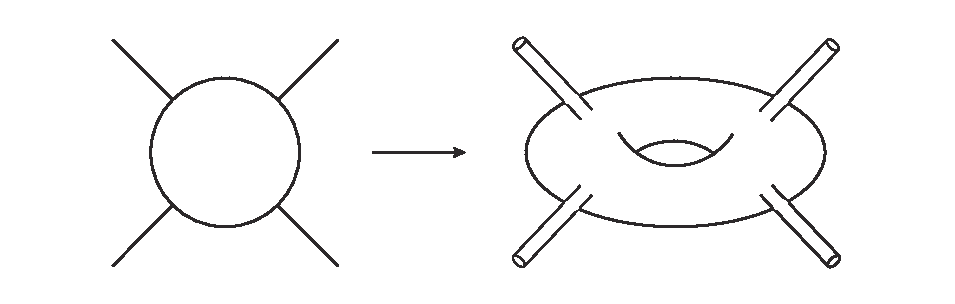
\includegraphics[width=250pt]{picture/fig1}}
 \caption{A Feynman diagram of QFT (left) and a string interaction diagram (right). Each end of the cylinders emanating from the torus (or a Riemann surface in general) in the string interaction diagram corresponds to an initial/final state.}
 \label{fig1}
\end{figure}
Each end of the cylinders in the Figure corresponds to an initial/final state of a string. The action \eqref{string-sigma} of the string sigma model is invariant under the world-sheet diffeomorphisms, and it is a conformal field theory as a result.
As we will see in the next section \S\ref{sec:2dcft}, one can make use of the \textbf{state-operator correspondence} in a 2d CFT.  Hence, instead of using the Hamiltonian formalism of string states,  we will use vertex operators $\wh V_i$ in the path integral formalism:
\begin{align}\nonumber
 A_n = \sum_g \int \left(\cD h_{ab}\right)_{g,n} \int \cD X^\mu e^{-S_\sigma [X^\mu,h_{ab}]} \wh V_1 \cdots \wh V_n \ ,
\end{align}
where $n$ is the number of in-coming/out-going strings, and $g$ is the number of holes(genus) of the Riemann surface (genus is $1$ in Figure \ref{fig2}). Here we integrate over all the metric $h_{ab}$ and field $X^\mu$ configuration up to gauge transformations, and we also sum over all the topology (genus $g$) of world-sheets.




\begin{figure}[htb]
 \centerline{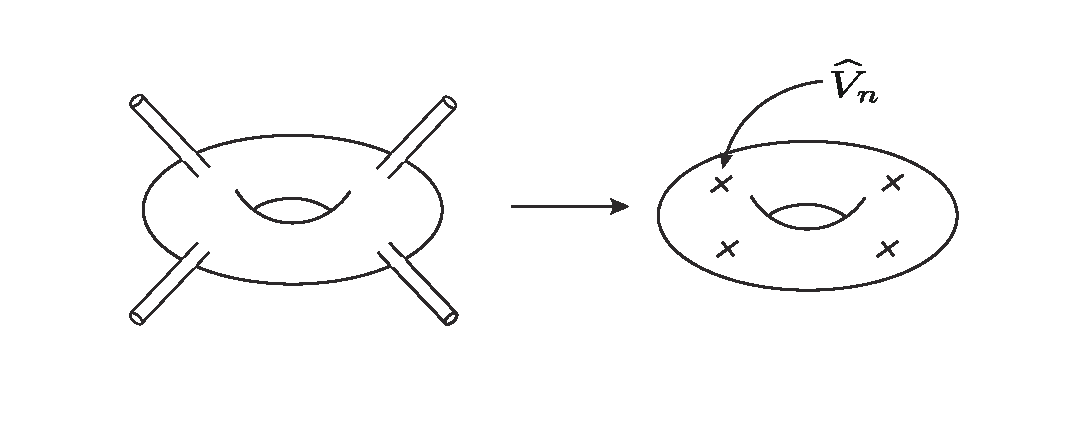
\includegraphics[width=250pt]{picture/fig2}}
 \caption{String interaction in state expression (left) and operator expression (right).}
 \label{fig2}
\end{figure}



In the path integral method, expectation values are schematically expressed in the following form
\begin{align}\nonumber
 \langle \mathcal O[X] \rangle = \int \cD X e^{iS[X]} \mathcal O [X] \ ,  \qquad
 S = \frac{1}{4\pi \alpha'} \int d\sigma d\tau \left\{ \left(\partial_\tau X\right)^2 -\left(\partial_\sigma X\right)^2\right\} \ ,
\end{align}
where $\mathcal O$ is a
gauge-invariant operator.


We usually \textbf{Wick rotate} ($\tau \to -it$) the theory so that it converges.
\begin{align}\nonumber
 \langle \mathcal O[X] \rangle = \int \cD X e^{-S_E[X]} \mathcal O [X] \ ,  \qquad
 S_E = \frac{1}{4\pi \alpha'} \int d\sigma dt \left\{ \left(\partial_t X\right)^2 +\left(\partial_\sigma X\right)^2\right\} \ .
\end{align}
The subscript $E$ will be omitted hereafter, and we will always work in the world-sheet Euclidean signature.




\end{document}
